\begin{figure}[H]
    \renewcommand{\figurename}{Рисунок}
    \centering{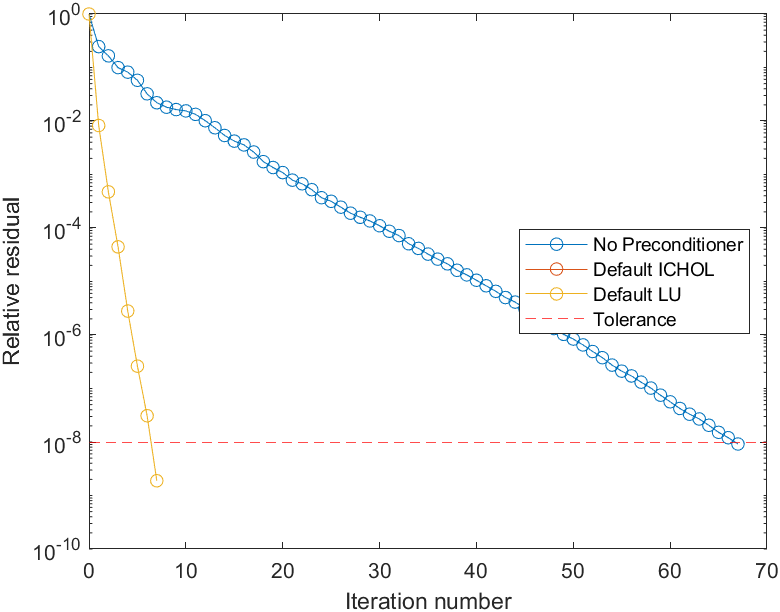
\includegraphics[scale=0.70, inner]{img/qa8fm/bicg}}
    \caption{История невязок методом bicg для матрицы Qa8fm}
    \label{fig:image_12}
\end{figure}

\begin{figure}[H]
    \renewcommand{\figurename}{Рисунок}
    \centering{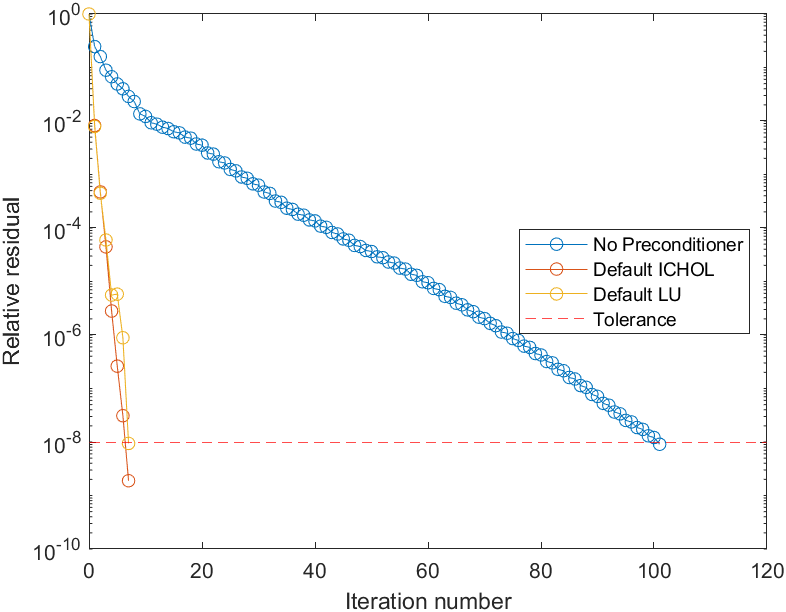
\includegraphics[scale=0.70]{img/qa8fm/bicgstab}}
    \caption{История невязок методом bicgstab для матрицы Qa8fm}
    \label{fig:image_13}
\end{figure}

\begin{figure}[H]
    \renewcommand{\figurename}{Рисунок}
    \centering{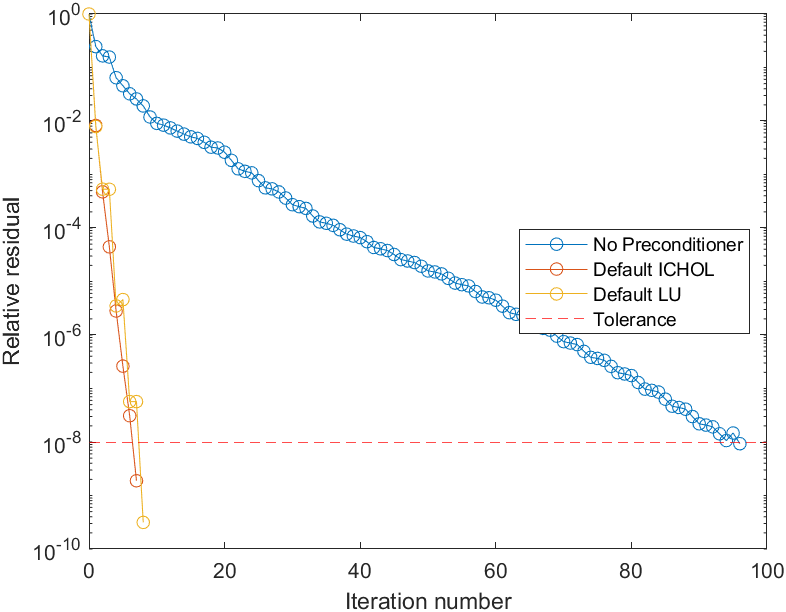
\includegraphics[scale=0.70]{img/qa8fm/bicgstabl}}
    \caption{История невязок методом bicgstabl для матрицы Qa8fm}
    \label{fig:image_14}
\end{figure}

\begin{figure}[H]
    \renewcommand{\figurename}{Рисунок}
    \centering{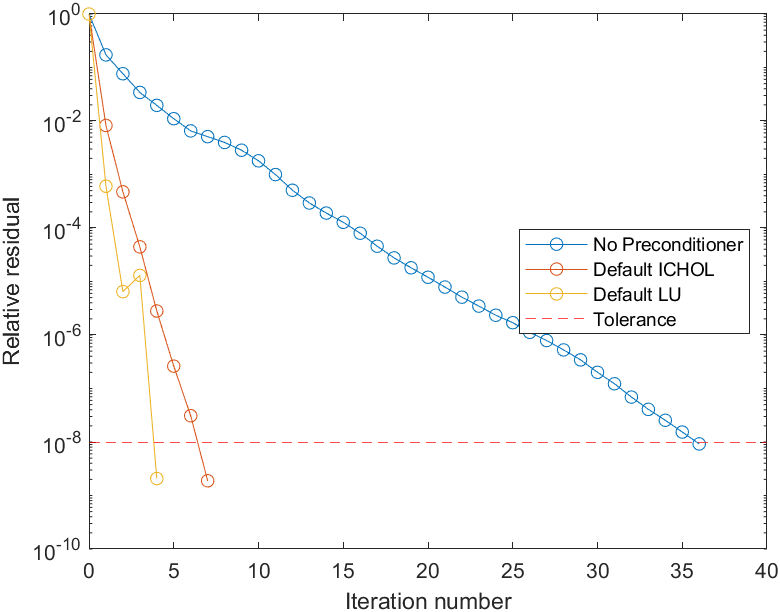
\includegraphics[scale=0.70]{img/qa8fm/cgs}}
    \caption{История невязок методом cgs для матрицы Qa8fm}
    \label{fig:image_15}
\end{figure}

\begin{figure}[H]
    \renewcommand{\figurename}{Рисунок}
    \centering{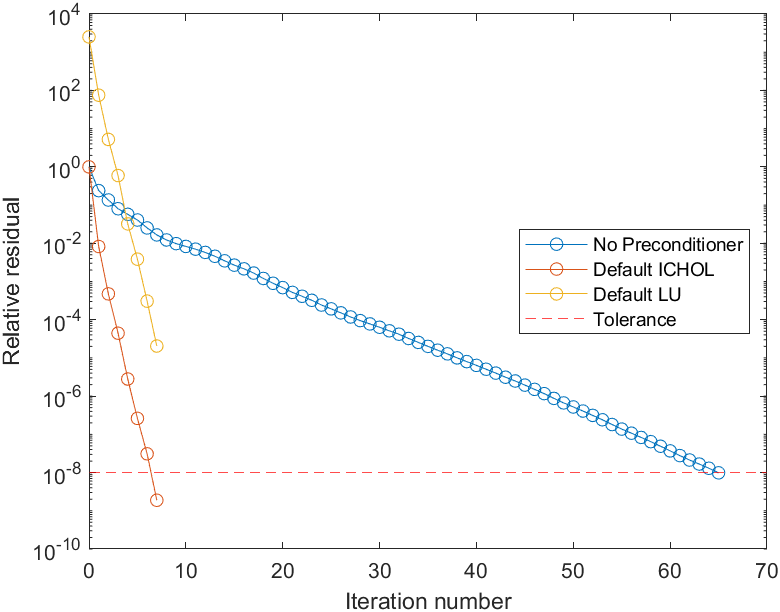
\includegraphics[scale=0.70]{img/qa8fm/gmres}}
    \caption{История невязок методом gmres для матрицы Qa8fm}
    \label{fig:image_16}
\end{figure}

\begin{figure}[H]
    \renewcommand{\figurename}{Рисунок}
    \centering{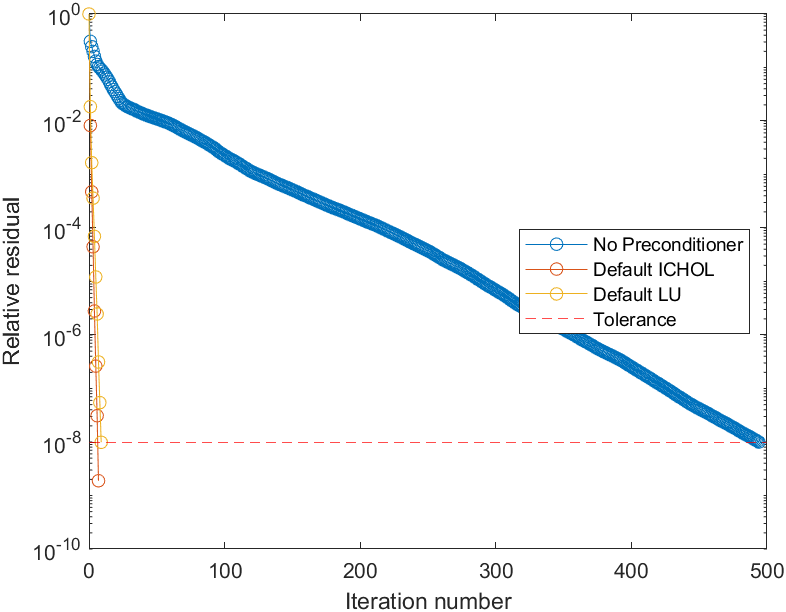
\includegraphics[scale=0.70]{img/qa8fm/lsqr}}
    \caption{История невязок методом lsqr для матрицы Qa8fm}
    \label{fig:image_17}
\end{figure}

\begin{figure}[H]
    \renewcommand{\figurename}{Рисунок}
    \centering{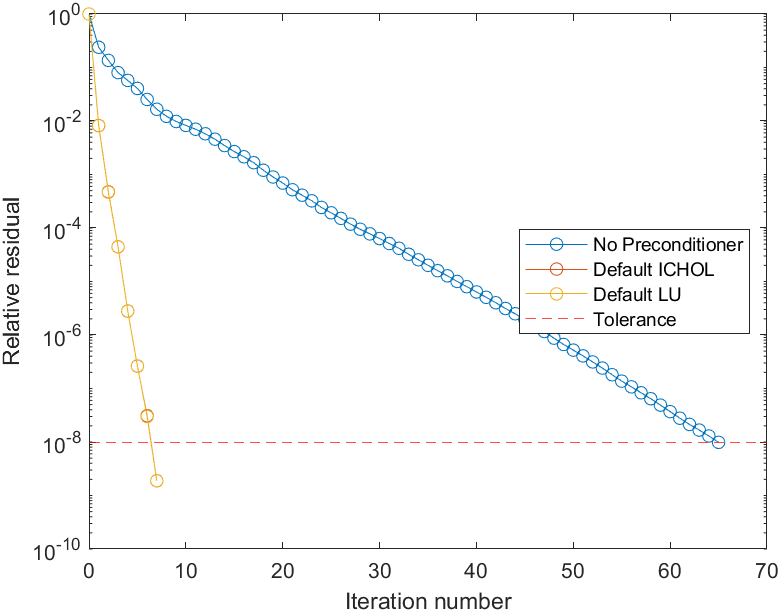
\includegraphics[scale=0.70]{img/qa8fm/minres}}
    \caption{История невязок методом minres для матрицы Qa8fm}
    \label{fig:image_18}
\end{figure}

\begin{figure}[H]
    \renewcommand{\figurename}{Рисунок}
    \centering{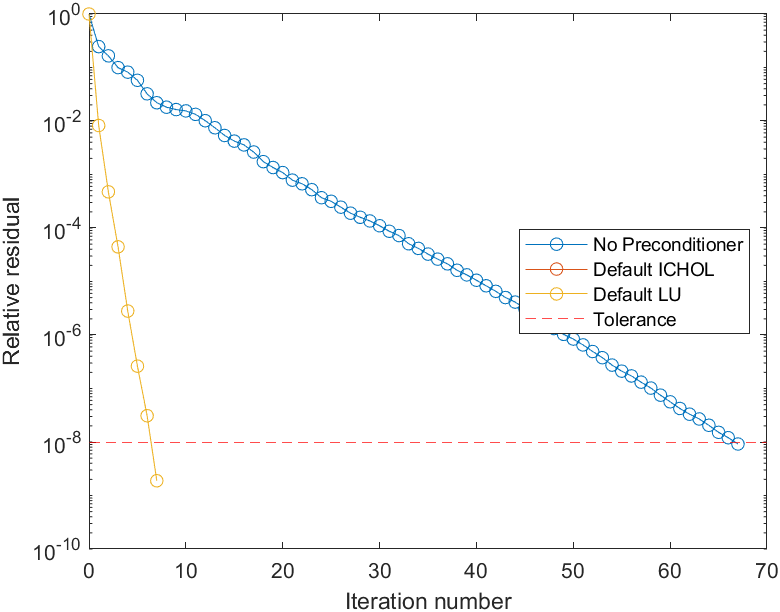
\includegraphics[scale=0.70]{img/qa8fm/pcg}}
    \caption{История невязок методом pcg для матрицы Qa8fm}
    \label{fig:image_19}
\end{figure}

\begin{figure}[H]
    \renewcommand{\figurename}{Рисунок}
    \centering{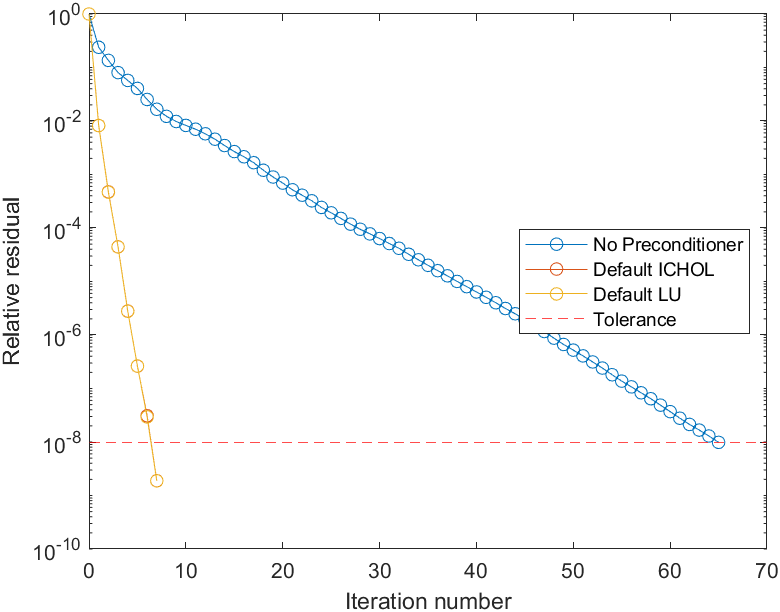
\includegraphics[scale=0.70]{img/qa8fm/qmr}}
    \caption{История невязок методом qmr для матрицы Qa8fm}
    \label{fig:image_20}
\end{figure}

\begin{figure}[H]
    \renewcommand{\figurename}{Рисунок}
    \centering{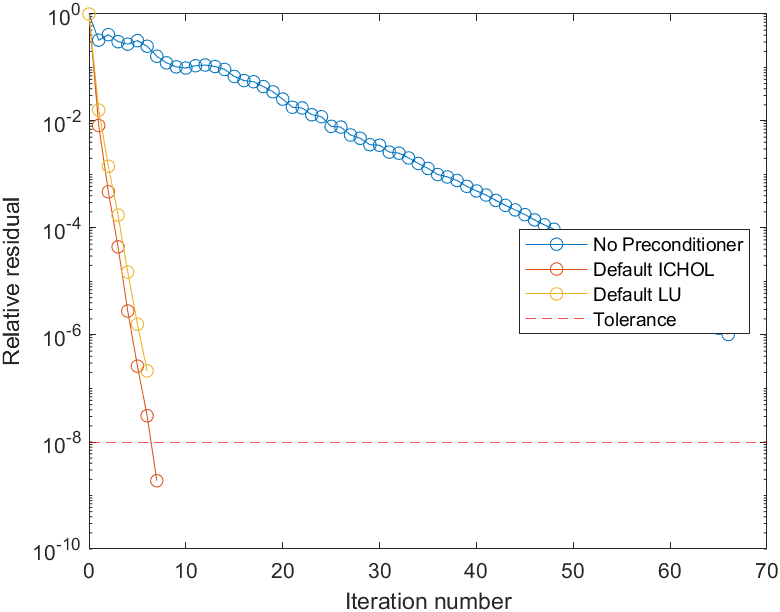
\includegraphics[scale=0.70]{img/qa8fm/symmlq}}
    \caption{История невязок методом symmlq для матрицы Qa8fm}
    \label{fig:image_21}
\end{figure}

\begin{figure}[H]
    \renewcommand{\figurename}{Рисунок}
    \centering{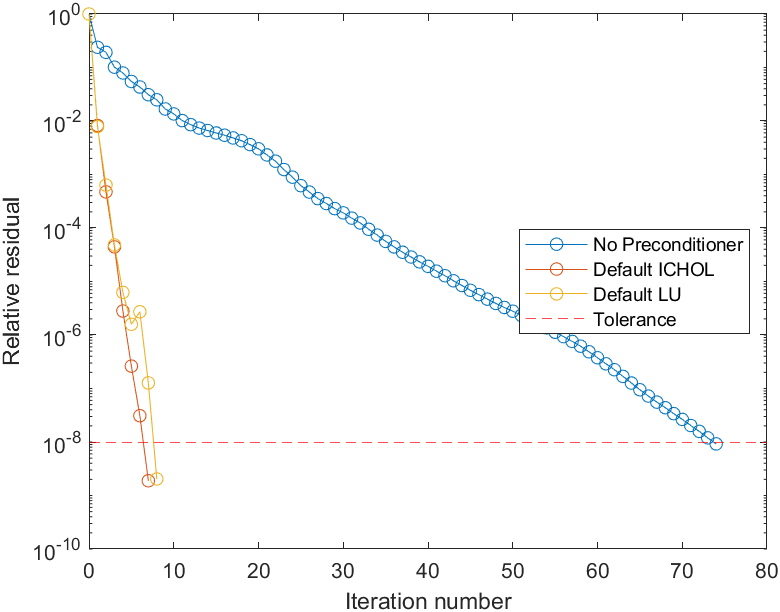
\includegraphics[scale=0.70]{img/qa8fm/tfqmr}}
    \caption{История невязок методом tfqmr для матрицы Qa8fm}
    \label{fig:image_22}
\end{figure}
